The Camera System Layer contains a camera subsystem, the gimbal subsystem, and signal controller subsystem. The camera subsystem streams the raw video feeds of the stereo cameras. The gimbal subsystem maintains the desired camera angles. The signal controller subsystem receives the angular data and controls the motor based on the data.

\begin{figure}[h!]
	\centering
 	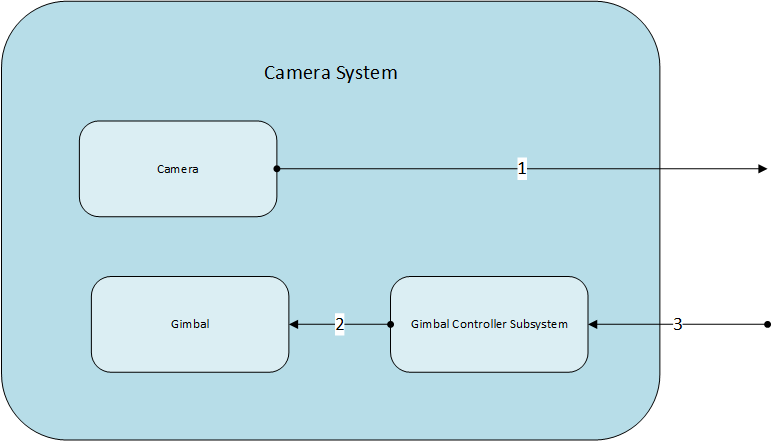
\includegraphics[width=0.60\textwidth]{images/camerasubsystem}
 \caption{Camera System Layer subsystem description diagram}
\end{figure}

\subsection{Layer Hardware}
The Camera System has many hardware components. The camera subsystem contains two wide-angle HD USB camera modules, ELP-USBFHD01M-L21. The gimbal subsystem contains three brushless motors, Rctimer GBM2804, and a custom 3D printed housing. The signal controller subsystem contains a motor control board, Storm32-BGC V1.3.

\subsection{Layer Operating System}
Windows 7 or newer

\subsection{Layer Software Dependencies}
Requires the width and height of the video resolution to be set before the cameras begin to start sending video feed.

\subsection{Camera Subsystem}
The camera subsystem receives input from the cameras and sends the video signal to the Processing System.

\subsubsection{Subsystem Hardware}
The camera modules mentioned above (model No: ELP-USBFHD01M-L21) will be used side-by-side, separated by about 65 mm to simulate the average distance between human eyes.

\subsubsection{Subsystem Operating System}
Supporting operating system: WinXP, Vista, Win7, Win8, Linux with UVC MAC-OS X 10.4.8 or later, Wince with UVC, Android 4.0 or above

\subsubsection{Subsystem Software Dependencies}
The video resolution of the cameras is required to be set before starting to send video feed to the video encoding subsystem in the Processing System.

% Anything?
\subsubsection{Subsystem Programming Languages}
None

\subsubsection{Subsystem Data Structures}
The video output of the camera modules is FMPEG with a user-specified frame rate and resolution per frame.

% Anything?
\subsubsection{Subsystem Data Processing}
None

\subsection{Gimbal Subsystem}
The gimbal subsystem is a custom built three axis gimbal with stereo camera mounts and external mounting plates.

\subsubsection{Subsystem Hardware}
There are three Rctimer GBM2804 motors and a custom 3D printed housing.

% Anything?
\subsubsection{Subsystem Operating System}
None

\subsubsection{Subsystem Software Dependencies}
The Rctimer motors rely on the PWM output of the Storm32-BGC board for angular instruction.

% Anything?
\subsubsection{Subsystem Programming Languages}
None

% Anything?
\subsubsection{Subsystem Data Structures}
None

% Anything?
\subsubsection{Subsystem Data Processing}
None

\subsection{Signal Controller Subsystem}
The signal controller subsystem receives a pulse width modulated signal representing the three angles that the camera should be aligned relative to the initialized position. This alignment is achieved through the use of two inertial measurement unit modules. The control board adjusts the motors to keep the gimbal in alignment.

\subsubsection{Subsystem Hardware}
There are three Rctimer GBM2804 motors, a custom 3D printed housing, a Storm32-BGC V1.3, and MPU6050 IMU.

\subsubsection{Subsystem Operating System}
The control board runs on configurable firmware. The version used was V0.90.

\subsubsection{Subsystem Software Dependencies}
The PWM signal must be a pulse between 1-2 ms with a 15ms period.

\subsubsection{Subsystem Programming Languages}
User specifications can be digitally sent to the Storm32-BGC board using OlliW's custom user interface which translates settings directly to assembly level programming of the onboard STM32F103RC MCU.

\subsubsection{Subsystem Data Structures}
The Storm32-BGC v1.3 utilizes a Futuba S-Bus for data communication across the board's components.

% Anything?
\subsubsection{Subsystem Data Processing}
None